% 本试卷单独编译时不显示页眉，保留页码。
\pagestyle{plain}

\begin{center}
  {\Large\bfseries 2026年普通高等学校招生全国统一考试（北京卷）\par}
  \vspace{0.5em}
  {\Large\bfseries 数\quad 学}
\end{center}

\noindent 姓名：\underline{\hspace{4cm}}\hfill 准考证号：\underline{\hspace{5cm}}

\medskip
\noindent 本试卷共6页，150分。考试时长120分钟。考生务必将答案答在答题卡上，在试卷上作答无效。考试结束后，将本试卷和答题卡一并交回。

\subsection*{第一部分（选择题\quad 共40分）}

\noindent\textbf{一、选择题}（本大题共10小题，每小题4分，共40分。在每小题列出的四个选项中，选出符合题目要求的一项。）

\noindent 1. 已知集合$M=\{x\mid-1<x<3\}$，$N=\{x\mid x\geqslant2\}$，则$M\cup N=$（\quad）
\begin{center}
\begin{tabular}{@{}p{0.47\textwidth}p{0.47\textwidth}@{}}
A. $\{x\mid x>-1\}$ & B. $\{x\mid x<3\}$ \\
C. $\{x\mid x\geqslant2\}$ & D. $\{x\mid2\leqslant x<3\}$
\end{tabular}
\end{center}

\noindent 2. 已知复数$z_1=3-2\mathrm{i}$，$z_2=-5+4\mathrm{i}$，则$|z_1+z_2|=$（\quad）
\begin{multicols}{4}
\begin{enumerate}[label=\Alph*.,leftmargin=*]
  \item $\sqrt2$
  \item $2$
  \item $2\sqrt2$
  \item $8$
\end{enumerate}
\end{multicols}

\noindent 3. 已知双曲线$\dfrac{x^2}{a^2}-\dfrac{y^2}{4}=1$（$a>0$）的渐近线方程为$y=\pm\dfrac23x$，则$a=$（\quad）
\begin{multicols}{4}
\begin{enumerate}[label=\Alph*.,leftmargin=*]
  \item $\sqrt3$
  \item $3$
  \item $6$
  \item $9$
\end{enumerate}
\end{multicols}

\noindent 4. 在$(a-\sqrt{x})^7$的展开式中，若$x^2$的系数为$280$，则实数$a=$（\quad）
\begin{multicols}{4}
\begin{enumerate}[label=\Alph*.,leftmargin=*]
  \item $2$
  \item $-2$
  \item $1$
  \item $-1$
\end{enumerate}
\end{multicols}

\noindent 5. 下列函数中，是奇函数且在其定义域上单调递增的为（\quad）
\begin{center}
\begin{tabular}{@{}p{0.47\textwidth}p{0.47\textwidth}@{}}
A. $y=\dfrac{1}{x^2+1}$ & B. $y=2^{-x}-2^x$ \\
C. $y=\sin x$ & D. $y=\ln\dfrac{5+x}{5-x}$
\end{tabular}
\end{center}

\noindent 6. 已知向量$\boldsymbol a,\boldsymbol b$满足$\boldsymbol a=(-3,0)$，$|\boldsymbol a-\boldsymbol b|=1$，则（\quad）
\begin{center}
\begin{tabular}{@{}p{0.47\textwidth}p{0.47\textwidth}@{}}
A. $|\boldsymbol b|$的最小值为$1$ & B. $|\boldsymbol b|$的最小值为$3$ \\
C. $|\boldsymbol b|$的最大值为$3$ & D. $|\boldsymbol b|$的最大值为$4$
\end{tabular}
\end{center}

\noindent 7. 已知$\{a_n\}$，$\{b_n\}$均为无穷数列，则“存在常数$M$，使得$a_n\leqslant M\leqslant b_n$（$n=1,2,\ldots$）”是“$a_n\leqslant b_n$（$n=1,2,\ldots$）”的（\quad）
\begin{center}
\begin{tabular}{@{}p{0.47\textwidth}p{0.47\textwidth}@{}}
A. 充分不必要条件 & B. 必要不充分条件 \\
C. 充要条件 & D. 既不充分也不必要条件
\end{tabular}
\end{center}

\noindent 8. 设函数$f(x)=\sin(x+\varphi)$（$0<\varphi<2\pi$）。若将$y=f(x)$的图象沿$x$轴的正方向平移$3\varphi$个单位长度，所得图象与$y=f(x)$的图象关于$x$轴对称，则满足条件的$\varphi$的个数为（\quad）
\begin{multicols}{4}
\begin{enumerate}[label=\Alph*.,leftmargin=*]
  \item $1$
  \item $2$
  \item $3$
  \item $4$
\end{enumerate}
\end{multicols}

\noindent 9. 为纪念红军长征胜利90周年，某校组织高一和高二两个年级的学生去甲、乙两个红色教育基地进行研学，每位学生选择其中一个基地参加。已知该校高一学生人数多于高二学生人数。若选择甲基地的学生人数多于选择乙基地的学生人数，则（\quad）
\begin{enumerate}[label=\Alph*.,leftmargin=2.2em]
  \item 选择甲基地的高一学生人数多于选择乙基地的高一学生人数
  \item 选择甲基地的高一学生人数多于选择乙基地的高二学生人数
  \item 选择甲基地的高二学生人数不多于选择乙基地的高一学生人数
  \item 选择甲基地的高二学生人数不多于选择乙基地的高二学生人数
\end{enumerate}

\noindent 10. 曲柄摇杆机构可以实现旋转运动与摆动运动的相互转化，被广泛应用于多个领域。已知从某曲柄摇杆机构中可抽象出如图所示的平面图形$ABCD$，其中$A,B$为定点，$C,D$为动点，$AB=4$，$BC=\dfrac52$，$CD=3$，$AD=1$，则$\cos\angle ABC$的取值范围是（\quad）

\begin{center}
\begin{minipage}{0.46\textwidth}
\begin{enumerate}[label=\Alph*.,leftmargin=*]
  \item $\left[\dfrac5{16},\dfrac{53}{80}\right]$
  \item $\left[\dfrac5{16},\dfrac{73}{80}\right]$
  \item $\left[\dfrac5{12},\dfrac{53}{80}\right]$
  \item $\left[\dfrac5{12},\dfrac{73}{80}\right]$
\end{enumerate}
\end{minipage}\hfill
\begin{minipage}{0.48\textwidth}
\centering
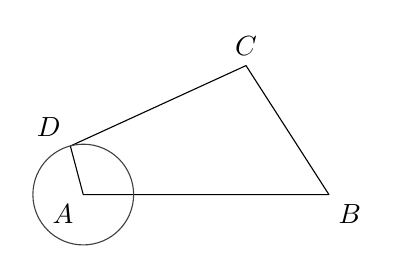
\begin{tikzpicture}[scale=0.78,line join=round,line cap=round]
  \coordinate (A) at (0,0);
  \coordinate (B) at (4,0);
  \coordinate (C) at (2.65,2.1);
  \coordinate (D) at (-0.21,0.79);
  \draw (A)--(B)--(C)--(D)--cycle;
  \draw[black!75] (A) circle (0.82);
  \foreach \P/\pos in {A/below left,B/below right,C/above,D/above left}
    \node[\pos] at (\P) {$\P$};
\end{tikzpicture}
\end{minipage}
\end{center}

\subsection*{第二部分（非选择题\quad 共110分）}

\noindent\textbf{二、填空题}（本大题共5小题，每小题5分，共25分。）

\noindent 11. 若直线$ax+y=0$与圆$(x-2)^2+(y-2)^2=4$相切，则$a=$\underline{\hspace{3cm}}.

\noindent 12. 已知公差为$d$的等差数列$\{a_n\}$的前$n$项和为$S_n$。若$S_6=6a_6+30$，则$d=$\underline{\hspace{2.5cm}}，使得$S_n\leqslant S_5$对所有$n$都成立的一个$a_1$的取值为\underline{\hspace{2.5cm}}.

\noindent 13. 我国在机器人技术领域取得了一系列重要成就。在处理机器人语音信号时，常用公式
\[
F(f)=k\lg\left(1+\frac{f}{700}\right)\quad(k>0)
\]
将声音频率$f$（单位：Hz）转换为$F(f)$。
\par\noindent 若$F(f)$的取值范围是
$[k\lg2,3k\lg2]$，则$f$的取值范围是\underline{\hspace{3cm}}.

\noindent 14. 如图，在三棱锥$A-BCD$中，$AB=AC=AD=2\sqrt2$，$BC=BD=2$，$CD=2\sqrt3$。该三棱锥的底面积为\underline{\hspace{2.5cm}}，体积为\underline{\hspace{2.5cm}}.

\begin{center}
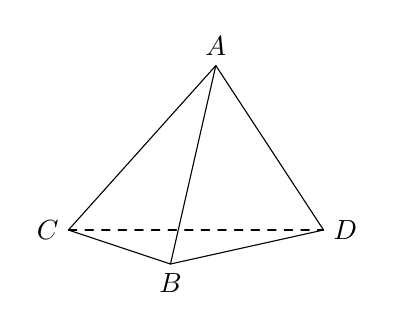
\begin{tikzpicture}[scale=0.72,line join=round,line cap=round]
  \coordinate (A) at (0.3,3.2);
  \coordinate (B) at (-0.5,-0.3);
  \coordinate (C) at (-2.3,0.3);
  \coordinate (D) at (2.2,0.3);
  \draw (A)--(B)--(C)--cycle;
  \draw (A)--(D)--(B);
  \draw[dashed] (C)--(D);
  \foreach \P/\pos in {A/above,B/below,C/left,D/right}
    \node[\pos] at (\P) {$\P$};
\end{tikzpicture}
\end{center}

\noindent 15. 已知$c$是非负常数，函数$f(x)=|x^2-\cos x-c^2|$。给出下列四个结论：

\noindent ①$f(x)$在区间$(-1,1]$上有最小值和最大值；

\noindent ②当$c=1$时，$f(x)$在区间$(1,2]$上有最大值；

\noindent ③当$c=0$时，方程$f(x)=1$的解集有3个元素；

\noindent ④当$c>0$时，方程$f(x)=c$的解集有4个元素。

\noindent 其中正确结论的序号是\underline{\hspace{3cm}}.

\newpage
\noindent\textbf{三、解答题}（本大题共6小题，共85分。解答应写出文字说明、演算步骤或证明过程。）

\noindent 16.（本小题13分）设函数
\[
f(x)=2\sin\omega x\cos\varphi+2\cos\omega x\sin\varphi
\quad\left(\omega>0,\ |\varphi|<\frac\pi2\right).
\]
已知$f(x)$的最小正周期为$\pi$，且$f\left(\dfrac\pi4\right)=1$，$f(0)>0$。

\noindent（I）求$\omega,\varphi$的值；

\noindent（II）求$f(x)$的单调递减区间.

\newpage
\noindent 17.（本小题13分）为了解某校高三年级学生的数学学习情况，随机抽查了200名高三年级学生某次考试的数学成绩，整理成下表：

\begin{center}
\renewcommand{\arraystretch}{1.45}
\setlength{\tabcolsep}{1.25em}
\begin{tabular}{|c|c|c|c|c|c|}
\hline
成绩&$[81,94)$&$[94,107)$&$[107,120)$&$[120,135)$&$[135,150]$\\ \hline
人数&40&60&60&32&8\\ \hline
\end{tabular}
\end{center}

\noindent 假设学生的数学成绩相互独立，用频率估计概率。

\noindent（I）估计该校高三年级学生这次考试的数学成绩低于120的概率；

\noindent（II）从该校高三年级学生中随机抽取4人，估计在这次考试中，2人的数学成绩不低于120且2人的数学成绩低于94的概率；

\noindent（III）为分析该校高三年级学生的数学学习情况，可采用三种方法：将样本中每名学生数学成绩所在区间的左端点值、中点值和右端点值视为该生的数学成绩。分别将这三种方法得到的三组数学成绩的方差记为$s_{\text{左}}^2$、$s_{\text{中}}^2$和$s_{\text{右}}^2$，判断$s_{\text{左}}^2$、$s_{\text{中}}^2$和$s_{\text{右}}^2$的大小关系。（结论不要求证明）.

\newpage
\noindent 18.（本小题14分）如图，在直三棱柱$ABC-A_1B_1C_1$中，$D,E$分别为$AC,A_1B_1$的中点，$AB=AC=2$，$\angle BAC=90^\circ$，$BB_1=\sqrt2$。

\noindent（I）求证：$DE\parallel$平面$BCC_1B_1$；

\noindent（II）设点$P$在$\triangle A_1B_1C_1$的内部，$PE\parallel B_1C_1$。再从条件①、条件②、条件③这三个条件中选择一个作为已知，使点$P$的位置唯一确定，求平面$PAD$与平面$PDE$夹角的余弦值。

\noindent 条件①：$PA=PD$；

\noindent 条件②：$PA\perp BC$；

\noindent 条件③：$BB_1\parallel$平面$PDE$。

\noindent 注：如果选择的条件不符合要求，第（II）问得0分；如果选择多个符合要求的条件分别解答，按第一个解答计分.

\begin{center}
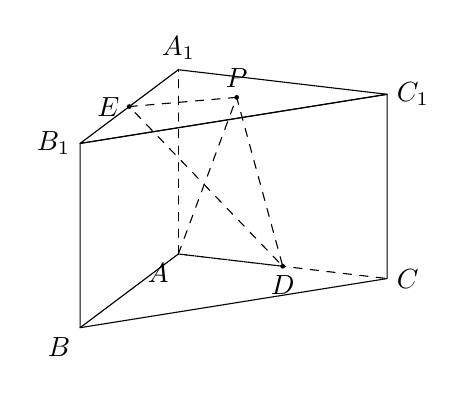
\begin{tikzpicture}[scale=0.78,line join=round,line cap=round]
  \coordinate (B)  at (-2.2,-1.2);
  \coordinate (A)  at (-0.6,0);
  \coordinate (C)  at (2.8,-0.4);
  \coordinate (B1) at (-2.2,1.8);
  \coordinate (A1) at (-0.6,3.0);
  \coordinate (C1) at (2.8,2.6);
  \coordinate (D)  at (1.1,-0.2);
  \coordinate (E)  at (-1.4,2.4);
  \coordinate (P)  at (0.35,2.55);
  \draw (B)--(C)--(C1)--(B1)--cycle;
  \draw (B)--(A);
  \draw (A1)--(B1)--(C1)--cycle;
  \draw[dashed] (A)--(C);
  \draw[dashed] (A)--(A1);
  \draw[dashed] (A)--(P)--(D)--cycle;
  \draw[dashed] (P)--(E)--(D);
  \fill (D) circle (1.1pt);
  \fill (E) circle (1.1pt);
  \fill (P) circle (1.1pt);
  \node[below left] at (A) {$A$};
  \node[below left] at (B) {$B$};
  \node[right] at (C) {$C$};
  \node[above] at (A1) {$A_1$};
  \node[left] at (B1) {$B_1$};
  \node[right] at (C1) {$C_1$};
  \node[below] at (D) {$D$};
  \node[left] at (E) {$E$};
  \node[above] at (P) {$P$};
\end{tikzpicture}
\end{center}

\newpage
\noindent 19.（本小题15分）已知椭圆$E:\dfrac{x^2}{a^2}+\dfrac{y^2}{b^2}=1$（$a>b>0$）的一个顶点为$(2,0)$，离心率为$\dfrac12$。过点$A(1,1)$且斜率为$k$（$k\neq\pm1$）的直线与椭圆$E$交于不同的两点$B,C$。点$B$关于直线$y=x$的对称点为$D$，直线$CD$与直线$y=x$交于点$Q$。设$\triangle ABQ$与$\triangle ACQ$的面积分别为$S_{\triangle ABQ}$与$S_{\triangle ACQ}$。

\noindent（I）求椭圆$E$的方程；

\noindent（II）若$\left|S_{\triangle ABQ}-S_{\triangle ACQ}\right|=\dfrac58$，求$k$的值.

\newpage
\noindent 20.（本小题15分）设函数$f(x)=x^2+mx-4\mathrm{e}^{nx-1}$（$n$是整数）。已知曲线$y=f(x)$在点$(-1,f(-1))$处的切线方程为
\[
4x+\mathrm{e}^2y+\mathrm{e}^2+8=0.
\]

\noindent（I）求$m,n$的值；

\noindent（II）求$f(x)$的极值点个数；

\noindent（III）求直线$l:y=kx-1$（$k>0$）与曲线$y=f(x)$的交点个数.

\newpage
\noindent 21.（本小题15分）设$A$是如下形式的$m$行$n$列的数表：

\begin{center}
\renewcommand{\arraystretch}{1.5}
\begin{tabular}{|c|c|c|c|}
\hline
$a_{11}$&$a_{12}$&$\cdots$&$a_{1n}$\\ \hline
$a_{21}$&$a_{22}$&$\cdots$&$a_{2n}$\\ \hline
$\vdots$&$\vdots$&$\ddots$&$\vdots$\\ \hline
$a_{m1}$&$a_{m2}$&$\cdots$&$a_{mn}$\\ \hline
\end{tabular}
\end{center}

其中位于第$i$行第$j$列的数记为$a_{ij}$，且$a_{ij}\in\{-1,1\}$（$i=1,2,\ldots,m$；$j=1,2,\ldots,n$）。

若对任意的$k,l\in\{1,2,\ldots,m\}$和$p,q\in\{1,2,\ldots,n\}$，当$l>k$，$q>p$且$(l-k)-(q-p)\in\{-2,2\}$时，均有
\[
a_{kp}+a_{kq}+a_{lp}+a_{lq}=0,
\]
则称数表$A$具有性质$P$。

\noindent（I）分别判断数表$A_1$和$A_2$是否具有性质$P$；（只需写出结论）

\begin{center}
$A_1=$\,
\begin{tabular}{|c|c|c|c|}
\hline 1&1&$-1$&1\\ \hline
$-1$&1&$-1$&1\\ \hline
\end{tabular}
\qquad\qquad
$A_2=$\,
\begin{tabular}{|c|c|c|c|}
\hline 1&$-1$&1&$-1$\\ \hline
1&1&$-1$&$-1$\\ \hline
$-1$&1&1&1\\ \hline
\end{tabular}
\end{center}

\noindent（II）当$m=4,n=5$时，若数表$A$具有性质$P$，求$A$中$1$的个数的最大值；

\noindent（III）当$m=n=6$时，若数表$A$具有性质$P$，且$a_{11}=1$，证明：
\[
a_{ij}=a_{i1}a_{1j}\qquad(i=1,2,\ldots,6;\ j=1,2,\ldots,6).
\]
